\paragraph*{Contenuto}
La pagina parla di FreedHome, il sistema di moduli e prodotti di Caccaro. Ancora troppe parole (più di 750), che consumano molto più tempo di quanto un utente sia disposto a spendere, come già visto in \fullref{sez:DualHome} e \fullref{sez:Home}. A differenza di quest'ultime, questa pagina si distingue per la concretezza e l'utilità delle informazioni presenti. I paragrafi, anche se in alcuni casi ripetitivi, rispondono alle domane \textit{"Cos'è?"}, \textit{"perché mi dovrebbe interessare?"}, e non proseguono nella solita retorica emotiva.\\
I paragrafi, inoltre, hanno titoli sensati e in grassetto, che aiutano l'utente a crearsi una mappa mentale in modo veloce e coerente. Male però che questi titoli non contengano link: sarebbe lecito aspettarsi, ad esempio, che cliccando su "Moduli" o sull'immagine adiacente si aprisse una pagina con la lista dei moduli.

\paragraph*{Scrolling}
Inutile ripetersi ulteriormente. Vedi \fullref{sez:DualHome_Scrolling}.

\paragraph*{Immagini}
Persistono i problemi già visti in precedenza dovuti all'elevata dimensione delle immagini.\\
Detto questo, per la maggior parte delle immagini nella pagina vale quanto detto per i paragrafi: il contenuto è significativo, seppur di minor importanza rispetto al testo che accompagna. Essendo il sistema FreedHome altamente configurabile, risulta vincente la scelta di mostrarne alcune configurazioni (non avrebbe senso scegliere una configurazione singola e mostrarla da ogni dettaglio). Le altre immagini rappresentano principalmente i singoli moduli, vari esempi di configurazione, e le finiture disponibili: bene, il tutto evidenzia la modularità del sistema.\\
Meno bene invece il video/GIF che accompagna il paragrafo \textit{Sistema FreedHome}. L'animazione, oltre a essere distraente per l'utente, non fornisce un valore aggiunto che la giustifichi (\autoref{fig:Animazione}).

\begin{figure}[H]
    \centering
    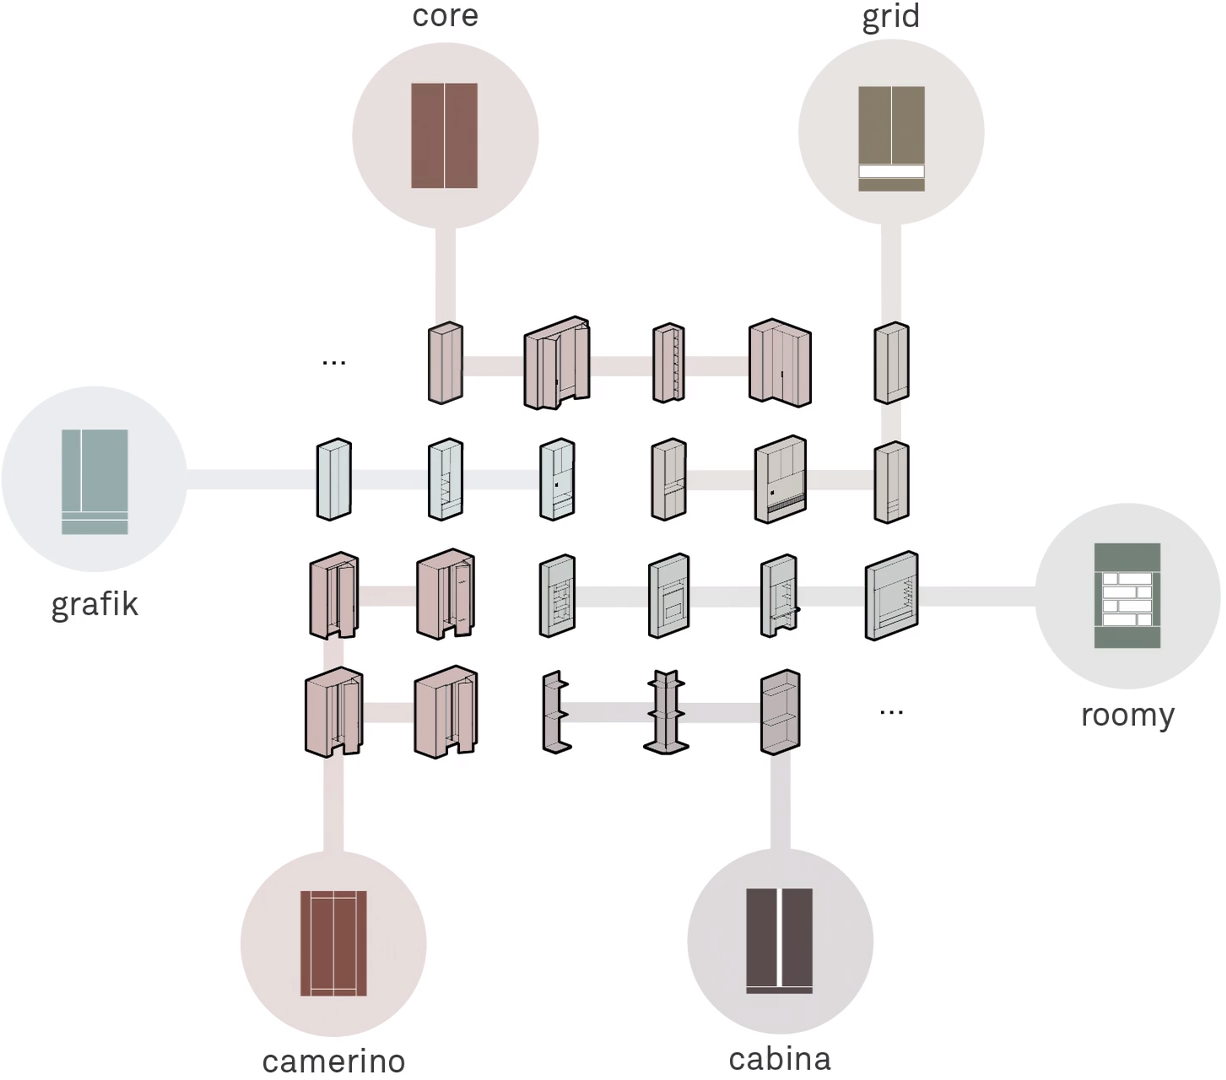
\includegraphics[width=10cm,keepaspectratio]{sez/FreedHome/img/video.png}
    \caption{Al posto dell'animazione, sarebbe bastata questa figura.}
    \label{fig:Animazione}
\end{figure}